% answers.tex —— 2000 年·全国旧课程卷·理科 · 参考答案与详细解析片段
% 由 tools/generate_projects.py 依来源总账自 2000/2000_数学真题_全国旧课程理_试题.md + 2000/2000_数学真题_全国旧课程理_解析正文.md + 2000/2000_数学真题_全国旧课程理_答案要点.md 生成，勿手改（改源 MD 后重跑）


\begin{gktip}
固定源 PDF 只有两页题面，没有答案和解析页。以下各题均依据题面独立复算；第 5、12、16、18、21、22 题的图形在 LaTeX 工程中以 TikZ/PGFPlots 矢量源重绘。
\end{gktip}

\gkpart{一、选择题}

\begin{answer}
\gksolhead{1}{}

\textbf{题目}：

设集合 $A$ 和 $B$ 都是自然数集合 $\mathbb N$，映射 $f:A\to B$ 把集合 $A$ 中的元素 $n$ 映射成集合 $B$ 中的元素 $2^n+n$，则在映射 $f$ 下，象 $20$ 的原象是\mbox{（　　）}

（A）2　　（B）3　　（C）4　　（D）5

\Needspace{4\baselineskip}
\textbf{解析}

\Needspace{5\baselineskip}
解方程

\nopagebreak[4]
\[
2^n+n=20.
\]

试得 $n=4$ 时等式成立，且函数 $2^n+n$ 在自然数上严格递增，所以原象为 $4$，选 C。

\gkanswer{答案：C}

\end{answer}
\begin{answer}
\gksolhead{2}{}

\textbf{题目}：

在复平面内，把复数 $3-\sqrt3\,i$ 对应的向量按顺时针方向旋转 $\dfrac\pi3$，所得向量对应的复数是\mbox{（　　）}

（A）$2\sqrt3$　　（B）$-2\sqrt3\,i$　　（C）$\sqrt3-3i$　　（D）$3+\sqrt3\,i$

\Needspace{4\baselineskip}
\textbf{解析}

\Needspace{5\baselineskip}
复数 $3-\sqrt3\,i$ 的模为 $2\sqrt3$，辐角为 $-\dfrac\pi6$。顺时针旋转 $\dfrac\pi3$ 后，辐角变为 $-\dfrac\pi2$，所以所得复数为

\nopagebreak[4]
\[
2\sqrt3\left(\cos\left(-\frac\pi2\right)+i\sin\left(-\frac\pi2\right)\right)
=-2\sqrt3\,i.
\]

选 B。

\gkanswer{答案：B}

\end{answer}
\begin{answer}
\gksolhead{3}{}

\textbf{题目}：

一个长方体共一顶点的三个面的面积分别是 $\sqrt2$、$\sqrt3$、$\sqrt6$，这个长方体对角线的长是\mbox{（　　）}

（A）$2\sqrt3$　　（B）$3\sqrt2$　　（C）6　　（D）$\sqrt6$

\Needspace{4\baselineskip}
\textbf{解析}

\Needspace{5\baselineskip}
设长方体三条棱长为 $x,y,z$，则

\nopagebreak[4]
\[
xy=\sqrt2,\qquad yz=\sqrt3,\qquad zx=\sqrt6.
\]

\Needspace{5\baselineskip}
于是

\nopagebreak[4]
\[
x^2=\frac{(xy)(xz)}{yz}=2,\qquad
y^2=1,\qquad z^2=3.
\]

\Needspace{5\baselineskip}
长方体对角线长为

\nopagebreak[4]
\[
\sqrt{x^2+y^2+z^2}=\sqrt6,
\]

选 D。

\gkanswer{答案：D}

\end{answer}
\begin{answer}
\gksolhead{4}{}

\textbf{题目}：

已知 $\sin\alpha>\sin\beta$，那么下列命题成立的是\mbox{（　　）}

（A）若 $\alpha$、$\beta$ 是第一象限角，则 $\cos\alpha>\cos\beta$

（B）若 $\alpha$、$\beta$ 是第二象限角，则 $\tan\alpha>\tan\beta$

（C）若 $\alpha$、$\beta$ 是第三象限角，则 $\cos\alpha>\cos\beta$

（D）若 $\alpha$、$\beta$ 是第四象限角，则 $\tan\alpha>\tan\beta$

\Needspace{4\baselineskip}
\textbf{解析}

在第四象限内，$\sin x$ 随角度增大而增大，$\tan x$ 也随角度增大而增大。因此 $\sin\alpha>\sin\beta$ 可推出 $\alpha>\beta$，进而 $\tan\alpha>\tan\beta$。这正是选项 D。

\gkanswer{答案：D}

\end{answer}
\begin{answer}
\gksolhead{5}{}

\textbf{题目}：

函数 $y=-x\cos x$ 的部分图象是\mbox{（　　）}
\nopagebreak[4]
\begin{center}% 2000 年全国旧课程卷理科第 5 题：y=-x cos x 的四个图象选项
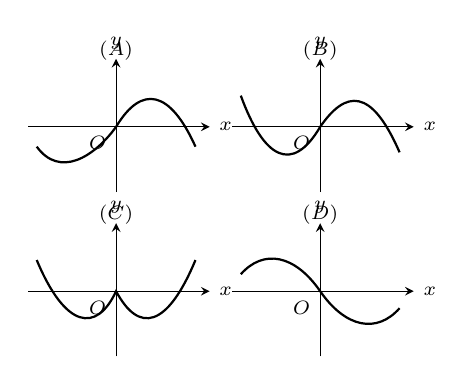
\begin{tikzpicture}[>=stealth, scale=0.72]
  \begin{scope}
    \node[font=\scriptsize] at (0,1.35) {$(A)$};
    \draw[->] (-1.55,0)--(1.65,0) node[right, font=\scriptsize] {$x$};
    \draw[->] (0,-1.15)--(0,1.2) node[above, font=\scriptsize] {$y$};
    \draw[thick] (-1.4,-0.35) .. controls (-1.0,-0.9) and (-0.4,-0.55) .. (0,0)
      .. controls (0.45,0.75) and (0.95,0.65) .. (1.4,-0.35);
    \node[below left, font=\scriptsize] at (0,0) {$O$};
  \end{scope}

  \begin{scope}[xshift=3.6cm]
    \node[font=\scriptsize] at (0,1.35) {$(B)$};
    \draw[->] (-1.55,0)--(1.65,0) node[right, font=\scriptsize] {$x$};
    \draw[->] (0,-1.15)--(0,1.2) node[above, font=\scriptsize] {$y$};
    \draw[thick] (-1.4,0.55) .. controls (-1.0,-0.55) and (-0.5,-0.85) .. (0,0)
      .. controls (0.45,0.65) and (0.9,0.7) .. (1.4,-0.45);
    \node[below left, font=\scriptsize] at (0,0) {$O$};
  \end{scope}

  \begin{scope}[yshift=-2.9cm]
    \node[font=\scriptsize] at (0,1.35) {$(C)$};
    \draw[->] (-1.55,0)--(1.65,0) node[right, font=\scriptsize] {$x$};
    \draw[->] (0,-1.15)--(0,1.2) node[above, font=\scriptsize] {$y$};
    \draw[thick] (-1.4,0.55) .. controls (-0.9,-0.65) and (-0.35,-0.75) .. (0,0)
      .. controls (0.4,-0.75) and (0.9,-0.65) .. (1.4,0.55);
    \node[below left, font=\scriptsize] at (0,0) {$O$};
  \end{scope}

  \begin{scope}[xshift=3.6cm,yshift=-2.9cm]
    \node[font=\scriptsize] at (0,1.35) {$(D)$};
    \draw[->] (-1.55,0)--(1.65,0) node[right, font=\scriptsize] {$x$};
    \draw[->] (0,-1.15)--(0,1.2) node[above, font=\scriptsize] {$y$};
    \draw[thick] (-1.4,0.3) .. controls (-1.0,0.75) and (-0.45,0.65) .. (0,0)
      .. controls (0.45,-0.65) and (1.0,-0.75) .. (1.4,-0.3);
    \node[below left, font=\scriptsize] at (0,0) {$O$};
  \end{scope}
\end{tikzpicture}
\end{center}
\nopagebreak[4]
\Needspace{4\baselineskip}
\textbf{解析}

\Needspace{5\baselineskip}
函数

\nopagebreak[4]
\[
y=-x\cos x
\]

是奇函数，且在 $x=0$ 附近，$x<0$ 时函数值为正、$x>0$ 时函数值为负；它还在 $\cos x=0$ 处与 $x$ 轴相交。四个图象中只有 D 符合，选 D。

\gkanswer{答案：D}

\end{answer}
\begin{answer}
\gksolhead{6}{}

\textbf{题目}：

《中华人民共和国个人所得税法》规定，公民全月工资、薪金所得不超过 800 元的部分不必纳税，超过 800 元的部分为全月应纳税所得额，此项税款按下表分段累进计算：

\begin{center}
\begin{tabular}{lr}
\toprule
全月应纳税所得额 & 税率 \\
\midrule
不超过 500 元的部分 & 5\% \\
超过 500 元至 2000 元的部分 & 10\% \\
超过 2000 元至 5000 元的部分 & 15\% \\
$\cdots$ & $\cdots$ \\
\bottomrule
\end{tabular}
\end{center}

某人一月份交纳此项税款 26.78 元，则他的当月工资、薪金所得介于\mbox{（　　）}

（A）800–900 元　　（B）900–1200 元

（C）1200–1500 元　　（D）1500–2800 元

\Needspace{4\baselineskip}
\textbf{解析}

\Needspace{5\baselineskip}
应纳税所得额为 $500$ 元时，税款为

\nopagebreak[4]
\[
500\times5\%=25\ \text{\text{元}}.
\]

\Needspace{5\baselineskip}
已交税款为 $26.78$ 元，超出部分为 $1.78$ 元，落在第二档，故第二档应纳税所得额为

\nopagebreak[4]
\[
\frac{1.78}{10\%}=17.8\ \text{\text{元}}.
\]

\Needspace{5\baselineskip}
所以总应纳税所得额为 $517.8$ 元，工资、薪金所得为

\nopagebreak[4]
\[
800+517.8=1317.8\ \text{\text{元}},
\]

介于 $1200$ 元和 $1500$ 元之间，选 C。

\gkanswer{答案：C}

\end{answer}
\begin{answer}
\gksolhead{7}{}

\textbf{题目}：

若 $a>b>1$，$P=\sqrt{\lg a\cdot\lg b}$，$Q=\dfrac12(\lg a+\lg b)$，$R=\lg\dfrac{a+b}{2}$，则\mbox{（　　）}

（A）$R<P<Q$　　（B）$P<Q<R$　　（C）$Q<P<R$　　（D）$P<R<Q$

\Needspace{4\baselineskip}
\textbf{解析}

\Needspace{5\baselineskip}
因为 $a>b>1$，所以 $\lg a,\lg b$ 为两个不相等的正数。由算术平均数不小于几何平均数，

\nopagebreak[4]
\[
P=\sqrt{\lg a\cdot\lg b}
<\frac{\lg a+\lg b}{2}=Q.
\]

\Needspace{5\baselineskip}
又由 $a\ne b$，

\nopagebreak[4]
\[
\frac{a+b}{2}>\sqrt{ab},
\]

\Needspace{5\baselineskip}
两边取常用对数得

\nopagebreak[4]
\[
R=\lg\frac{a+b}{2}
>\frac{\lg a+\lg b}{2}=Q.
\]

因此 $P<Q<R$，选 B。

\gkanswer{答案：B}

\end{answer}
\begin{answer}
\gksolhead{8}{}

\textbf{题目}：

以极坐标系中的点 $(1,1)$ 为圆心，1 为半径的圆的方程是\mbox{（　　）}

（A）$\rho=2\cos\left(\theta-\dfrac\pi4\right)$　　（B）$\rho=2\sin\left(\theta-\dfrac\pi4\right)$

（C）$\rho=2\cos(\theta-1)$　　（D）$\rho=2\sin(\theta-1)$

\Needspace{4\baselineskip}
\textbf{解析}

\Needspace{5\baselineskip}
在极坐标系中，点 $(1,1)$ 表示距离极点为 $1$、极角为 $1$ 的点。设动点为 $(\rho,\theta)$，圆心距为 $1$、半径为 $1$，由余弦定理

\nopagebreak[4]
\[
\rho^2+1-2\rho\cos(\theta-1)=1.
\]

\Needspace{5\baselineskip}
除去极坐标表达中的公共因子 $\rho$，圆的方程为

\nopagebreak[4]
\[
\rho=2\cos(\theta-1),
\]

选 C。

\gkanswer{答案：C}

\end{answer}
\begin{answer}
\gksolhead{9}{}

\textbf{题目}：

一个圆柱的侧面展开图是一个正方形，这个圆柱的全面积与侧面积的比是\mbox{（　　）}

（A）$\dfrac{1+2\pi}{2\pi}$　　（B）$\dfrac{1+4\pi}{4\pi}$　　（C）$\dfrac{1+2\pi}{\pi}$　　（D）$\dfrac{1+4\pi}{2\pi}$

\Needspace{4\baselineskip}
\textbf{解析}

\Needspace{5\baselineskip}
设圆柱底面半径为 $r$、高为 $h$。侧面展开为正方形，所以

\nopagebreak[4]
\[
h=2\pi r.
\]

\Needspace{5\baselineskip}
侧面积为 $h^2$，两个底面面积为 $2\pi r^2=h^2/(2\pi)$，故全面积与侧面积之比为

\nopagebreak[4]
\[
\frac{h^2+\frac{h^2}{2\pi}}{h^2}
=\frac{1+2\pi}{2\pi}.
\]

选 A。

\gkanswer{答案：A}

\end{answer}
\begin{answer}
\gksolhead{10}{}

\textbf{题目}：

过原点的直线与圆 $x^2+y^2+4x+3=0$ 相切，若切点在第三象限，则该直线的方程是\mbox{（　　）}

（A）$y=\sqrt3x$　　（B）$y=-\sqrt3x$　　（C）$y=\dfrac{\sqrt3}{3}x$　　（D）$y=-\dfrac{\sqrt3}{3}x$

\Needspace{4\baselineskip}
\textbf{解析}

\Needspace{5\baselineskip}
圆

\nopagebreak[4]
\[
x^2+y^2+4x+3=0
\Longleftrightarrow
(x+2)^2+y^2=1
\]

\Needspace{5\baselineskip}
的圆心为 $(-2,0)$、半径为 $1$。设过原点的切线为 $y=kx$，则圆心到该直线的距离满足

\nopagebreak[4]
\[
\frac{|{-2k}|}{\sqrt{k^2+1}}=1,
\qquad k=\pm\frac{\sqrt3}{3}.
\]

\Needspace{5\baselineskip}
取正斜率时切点位于第三象限，故直线为

\nopagebreak[4]
\[
y=\frac{\sqrt3}{3}x.
\]

选 C。

\gkanswer{答案：C}

\end{answer}
\begin{answer}
\gksolhead{11}{}

\textbf{题目}：

过抛物线 $y=ax^2\ (a>0)$ 的焦点 $F$ 作一直线交抛物线于 $P$、$Q$ 两点，若线段 $PF$ 与 $FQ$ 的长分别是 $p$、$q$，则 $\dfrac1p+\dfrac1q$ 等于\mbox{（　　）}

（A）$2a$　　（B）$\dfrac1{2a}$　　（C）$4a$　　（D）$\dfrac4a$

\Needspace{4\baselineskip}
\textbf{解析}

\Needspace{5\baselineskip}
设抛物线为 $y=ax^2$，焦点为 $F$。过焦点的直线可写成

\nopagebreak[4]
\[
y=mx+\frac1{4a}.
\]

\Needspace{5\baselineskip}
与抛物线联立，交点横坐标 $x_1,x_2$ 满足

\nopagebreak[4]
\[
ax^2-mx-\frac1{4a}=0.
\]

\Needspace{5\baselineskip}
两根异号，且

\nopagebreak[4]
\[
|x_1-x_2|=\frac{\sqrt{m^2+1}}a,\qquad
|x_1x_2|=\frac1{4a^2}.
\]

\Needspace{5\baselineskip}
沿该直线的距离要乘以 $\sqrt{m^2+1}$，所以

\nopagebreak[4]
\[
p+q=\frac{m^2+1}{a},\qquad
pq=\frac{m^2+1}{4a^2}.
\]

\Needspace{5\baselineskip}
因此

\nopagebreak[4]
\[
\frac1p+\frac1q=\frac{p+q}{pq}=4a,
\]

选 C。

\gkanswer{答案：C}

\end{answer}
\begin{answer}
\gksolhead{12}{}

\textbf{题目}：

如图，$OA$ 是圆锥底面中心 $O$ 到母线的垂线，$OA$ 绕轴旋转一周所得曲面将圆锥分成体积相等的两部分，则母线与轴的夹角为\mbox{（　　）}
\nopagebreak[4]
\begin{center}% 2000 年全国旧课程卷理科第 12 题：圆锥轴截面与 OA
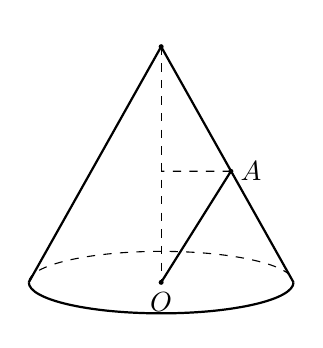
\begin{tikzpicture}[>=stealth, scale=0.82]
  \coordinate (V) at (0,3.65);
  \coordinate (O) at (0,0);
  \coordinate (L) at (-2.05,0);
  \coordinate (R) at (2.05,0);
  \coordinate (A) at (1.08,1.72);
  \draw[thick] (V)--(L) (V)--(R);
  \draw[thick] (L) arc (180:360:2.05 and 0.48);
  \draw[dashed] (L) arc (180:0:2.05 and 0.48);
  \draw[dashed] (V)--(O);
  \draw[thick] (O)--(A);
  \draw[dashed] (A)--(0,1.72);
  \fill (V) circle (1.1pt);
  \fill (O) circle (1.1pt) node[below] {$O$};
  \fill (A) circle (1.1pt) node[right] {$A$};
  \node[above] at (V) { };
\end{tikzpicture}
\end{center}
\nopagebreak[4]
（A）$\arccos\dfrac1{\sqrt[3]{2}}$　　（B）$\arccos\dfrac12$　　（C）$\arccos\dfrac1{\sqrt2}$　　（D）$\arccos\dfrac1{\sqrt[4]{2}}$

\Needspace{4\baselineskip}
\textbf{解析}

\Needspace{5\baselineskip}
设母线与轴的夹角为 $\theta$。在圆锥的轴截面中使用垂线与投影的相似关系：若以 $OA$ 表示题图中的垂距，则原圆锥底面半径与旋转曲面所对应的截面半径分别可写为

\nopagebreak[4]
\[
\frac{OA}{\cos\theta}
\quad\text{\text{和}}\quad
OA\cos\theta.
\]

\Needspace{5\baselineskip}
旋转曲面把圆锥分成体积相等的两部分，轴截面中的等体积关系化为

\nopagebreak[4]
\[
\frac13\pi(OA\cos\theta)^2h
=\frac12\cdot\frac13\pi\left(\frac{OA}{\cos\theta}\right)^2h.
\]

\Needspace{5\baselineskip}
约去公共因子，得

\nopagebreak[4]
\[
\cos^4\theta=\frac12.
\]

\Needspace{5\baselineskip}
由于 $\theta$ 为锐角，

\nopagebreak[4]
\[
\cos\theta=\frac1{\sqrt[4]{2}},
\]

故选 D。

\gkanswer{答案：D}

\end{answer}
\gkpart{二、填空题}

\begin{answer}
\gksolhead{13}{}

\textbf{题目}：

乒乓球队的 10 名队员中有 3 名主力队员，派 5 名参加比赛，3 名主力队员要安排在第一、三、五位置，其余 7 名队员选 2 名安排在第二、四位置，那么不同的出场安排共有\gkblank{}种（用数字作答）。

\Needspace{4\baselineskip}
\textbf{解析}

\Needspace{5\baselineskip}
先把 3 名主力队员安排在第一、三、五位置，有 $3!$ 种；再从其余 7 人中选 2 人并安排在第二、四位置，有

\nopagebreak[4]
\[
\binom72\cdot2!=7\cdot6
\]

\Needspace{5\baselineskip}
种。因此总数为

\nopagebreak[4]
\[
3!\binom72 2!=6\cdot42=252.
\]

\gkanswer{答案：252}

\end{answer}
\begin{answer}
\gksolhead{14}{}

\textbf{题目}：

椭圆 $\dfrac{x^2}{9}+\dfrac{y^2}{4}=1$ 的焦点 $F_1,F_2$，点 $P$ 为其上的动点，当 $\angle F_1PF_2$ 为钝角时，点 $P$ 横坐标的取值范围是\gkblank{}。

\Needspace{4\baselineskip}
\textbf{解析}

\Needspace{5\baselineskip}
椭圆的焦点为 $(\pm\sqrt5,0)$。点 $P=(x,y)$ 时，

\nopagebreak[4]
\[
\overrightarrow{PF_1}\cdot\overrightarrow{PF_2}
=x^2+y^2-5.
\]

\Needspace{5\baselineskip}
角 $F_1PF_2$ 为钝角等价于该内积小于 $0$，即 $x^2+y^2<5$。又

\nopagebreak[4]
\[
y^2=4\left(1-\frac{x^2}{9}\right),
\]

\Needspace{5\baselineskip}
所以

\nopagebreak[4]
\[
x^2+4-\frac{4x^2}{9}<5
\Longleftrightarrow
x^2<\frac95.
\]

\Needspace{5\baselineskip}
故横坐标范围为

\nopagebreak[4]
\[
-\frac3{\sqrt5}<x<\frac3{\sqrt5}.
\]

\gkanswer{答案：$\left(-\dfrac3{\sqrt5},\dfrac3{\sqrt5}\right)$}

\end{answer}
\begin{answer}
\gksolhead{15}{}

\textbf{题目}：

\Needspace{5\baselineskip}
设 $\{a_n\}$ 是首项为 1 的正项数列，且

\nopagebreak[4]
\[
(n+1)a_{n+1}^2-na_n^2+a_{n+1}a_n=0
\qquad(n=1,2,3,\ldots),
\]

则它的通项公式是 $a_n=$\gkblank{}。

\Needspace{4\baselineskip}
\textbf{解析}

\Needspace{5\baselineskip}
原递推式为

\nopagebreak[4]
\[
(n+1)a_{n+1}^2-na_n^2+a_{n+1}a_n=0.
\]

\Needspace{5\baselineskip}
令 $r_n=a_{n+1}/a_n>0$，可得

\nopagebreak[4]
\[
(n+1)r_n^2+r_n-n=0.
\]

\Needspace{5\baselineskip}
该方程的正根为

\nopagebreak[4]
\[
r_n=\frac{n}{n+1}.
\]

\Needspace{5\baselineskip}
由 $a_1=1$，

\nopagebreak[4]
\[
a_n=\prod_{k=1}^{n-1}\frac{k}{k+1}=\frac1n.
\]

\gkanswer{答案：$a_n=\dfrac1n$}

\end{answer}
\begin{answer}
\gksolhead{16}{}

\textbf{题目}：

如图，$E$、$F$ 分别为正方体面 $ADD_1A_1$、面 $BCC_1B_1$ 的中心，则四边形 $BFD_1E$ 在该正方体的面上的射影可能是\gkblank{}。（要求：把可能的图序号都填上）
\nopagebreak[4]
\begin{center}% 2000 年全国旧课程卷理科第 16 题：正方体内四边形投影的可能图形
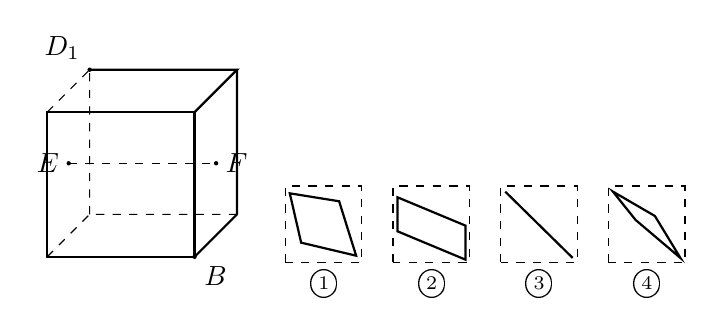
\begin{tikzpicture}[>=stealth, scale=0.72]
  \coordinate (A) at (0,0);
  \coordinate (B) at (2.6,0);
  \coordinate (C) at (3.35,0.75);
  \coordinate (D) at (0.75,0.75);
  \coordinate (A1) at (0,2.55);
  \coordinate (B1) at (2.6,2.55);
  \coordinate (C1) at (3.35,3.3);
  \coordinate (D1) at (0.75,3.3);
  \coordinate (E) at (0.38,1.65);
  \coordinate (F) at (2.98,1.65);

  \draw[thick] (A)--(B)--(B1)--(A1)--cycle;
  \draw[thick] (B1)--(C1)--(D1);
  \draw[dashed] (A)--(D)--(C) (D)--(D1) (A1)--(D1);
  \draw[thick] (B)--(C) (C)--(C1);
  \draw[dashed] (E)--(F);
  \fill (B) circle (1.1pt) node[below right] {$B$};
  \fill (D1) circle (1.1pt) node[above left] {$D_1$};
  \fill (E) circle (1.1pt) node[left] {$E$};
  \fill (F) circle (1.1pt) node[right] {$F$};

  \begin{scope}[xshift=4.2cm,yshift=-0.1cm]
    \draw[dashed] (0,0) rectangle (1.35,1.35);
    \draw[thick] (0.08,1.22)--(0.95,1.08)--(1.25,0.12)--(0.28,0.35)--cycle;
    \node[below] at (0.68,-0.08) {$\textcircled{\scriptsize 1}$};
  \end{scope}
  \begin{scope}[xshift=6.1cm,yshift=-0.1cm]
    \draw[dashed] (0,0) rectangle (1.35,1.35);
    \draw[thick] (0.08,1.15)--(0.08,0.55)--(1.28,0.05)--(1.28,0.65)--cycle;
    \node[below] at (0.68,-0.08) {$\textcircled{\scriptsize 2}$};
  \end{scope}
  \begin{scope}[xshift=8.0cm,yshift=-0.1cm]
    \draw[dashed] (0,0) rectangle (1.35,1.35);
    \draw[thick] (0.08,1.25)--(1.27,0.08);
    \node[below] at (0.68,-0.08) {$\textcircled{\scriptsize 3}$};
  \end{scope}
  \begin{scope}[xshift=9.9cm,yshift=-0.1cm]
    \draw[dashed] (0,0) rectangle (1.35,1.35);
    \draw[thick] (0.08,1.25)--(0.48,0.75)--(1.27,0.08)--(0.82,0.82)--cycle;
    \node[below] at (0.68,-0.08) {$\textcircled{\scriptsize 4}$};
  \end{scope}
\end{tikzpicture}
\end{center}
\nopagebreak[4]
\Needspace{4\baselineskip}
\textbf{解析}

\Needspace{5\baselineskip}
取正方体坐标为 $[0,1]^3$，令

\nopagebreak[4]
\[
B=(1,0,0),\quad D_1=(0,1,1),\quad
E=\left(0,\frac12,\frac12\right),\quad
F=\left(1,\frac12,\frac12\right).
\]

投影到含 $x$ 轴的两个相对面时，$B,F,D_1,E$ 的像退化为一条对角线，得到图③；投影到其余四个面时，四个像点组成同一个平行四边形，得到图②。因此可能的图序号为②③。

\gkanswer{答案：②③}

\end{answer}
\gkpart{三、解答题}

\begin{answer}
\gksolhead{17}{}

\textbf{题目}：

\Needspace{5\baselineskip}
已知函数

\nopagebreak[4]
\[
y=\sqrt3\sin x+\cos x,\qquad x\in\mathbb R.
\]

（1） 当函数 $y$ 取得最大值时，求自变量 $x$ 的集合；

（2） 该函数的图象可由 $y=\sin x\ (x\in\mathbb R)$ 的图象经过怎样的平移和伸缩变换得到？

\Needspace{4\baselineskip}
\textbf{解析}

\gksubpart{(1)}

\Needspace{5\baselineskip}
由

\nopagebreak[4]
\[
y=\sqrt3\sin x+\cos x
=2\sin\left(x+\frac\pi6\right),
\]

\Needspace{5\baselineskip}
函数最大值为 $2$，当且仅当

\nopagebreak[4]
\[
x+\frac\pi6=\frac\pi2+2k\pi,
\qquad k\in\mathbb Z.
\]

\Needspace{5\baselineskip}
所以

\nopagebreak[4]
\[
x=\frac\pi3+2k\pi,\qquad k\in\mathbb Z.
\]

\gksubpart{(2)}

\Needspace{5\baselineskip}
先把 $y=\sin x$ 的图象沿 $x$ 轴负向平移 $\dfrac\pi6$，得到

\nopagebreak[4]
\[
y=\sin\left(x+\frac\pi6\right);
\]

\Needspace{5\baselineskip}
再将纵坐标伸长为原来的 $2$ 倍，即得到

\nopagebreak[4]
\[
y=2\sin\left(x+\frac\pi6\right).
\]

\gkanswer{答案（1）：$x=\dfrac\pi3+2k\pi\ (k\in\mathbb Z)$。}

\gkanswer{答案（2）：先将 $y=\sin x$ 的图象沿 $x$ 轴负向平移 $\dfrac\pi6$，再将纵坐标伸长为原来的 2 倍。}

\end{answer}
\begin{answer}
\gksolhead{18}{}

\textbf{题目}：

\Needspace{5\baselineskip}
如图，已知平行六面体 $ABCD-A_1B_1C_1D_1$ 的底面 $ABCD$ 是菱形，且

\nopagebreak[4]
\[
\angle C_1CB=\angle C_1CD=\angle BCD=60^\circ.
\]

（1） 证明：$C_1C\perp BD$；

（2） 假定 $CD=2$，$CC_1=\dfrac32$，记面 $C_1BD$ 为 $\alpha$，面 $CBD$ 为 $\beta$，求二面角 $\alpha-BD-\beta$ 的平面角的余弦值；

（3） 当 $\dfrac{CD}{CC_1}$ 的值为多少时，能使 $A_1C\perp$ 平面 $C_1BD$？请给出证明。
\nopagebreak[4]
\begin{center}% 2000 年全国旧课程卷理科第 18 题：平行六面体 ABCD-A_1B_1C_1D_1
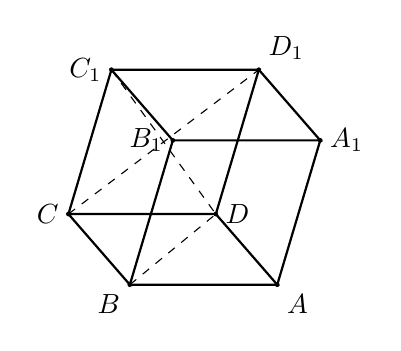
\begin{tikzpicture}[>=stealth, scale=0.78]
  \coordinate (A) at (3.4,0);
  \coordinate (B) at (1.0,0);
  \coordinate (C) at (0,1.15);
  \coordinate (D) at (2.4,1.15);
  \coordinate (A1) at (4.1,2.35);
  \coordinate (B1) at (1.7,2.35);
  \coordinate (C1) at (0.7,3.5);
  \coordinate (D1) at (3.1,3.5);

  \draw[thick] (A)--(B)--(C)--(D)--cycle;
  \draw[thick] (A1)--(B1)--(C1)--(D1)--cycle;
  \draw[thick] (A)--(A1) (B)--(B1) (C)--(C1) (D)--(D1);
  \draw[dashed] (C1)--(D) (B)--(D) (C)--(D1);

  \fill (A) circle (1.1pt) node[below right] {$A$};
  \fill (B) circle (1.1pt) node[below left] {$B$};
  \fill (C) circle (1.1pt) node[left] {$C$};
  \fill (D) circle (1.1pt) node[right] {$D$};
  \fill (A1) circle (1.1pt) node[right] {$A_1$};
  \fill (B1) circle (1.1pt) node[left] {$B_1$};
  \fill (C1) circle (1.1pt) node[left] {$C_1$};
  \fill (D1) circle (1.1pt) node[above right] {$D_1$};
\end{tikzpicture}
\end{center}
\nopagebreak[4]
\Needspace{4\baselineskip}
\textbf{解析}

\gksubpart{(1)}

\Needspace{5\baselineskip}
令 $C$ 为原点，取

\nopagebreak[4]
\[
\overrightarrow{CB}=\mathbf b,\qquad
\overrightarrow{CD}=\mathbf d,\qquad
\overrightarrow{CC_1}=\mathbf v.
\]

\Needspace{5\baselineskip}
由底面为菱形且 $\angle BCD=60^\circ$，

\nopagebreak[4]
\[
|\mathbf b|=|\mathbf d|,\qquad
\mathbf b\cdot\mathbf d=|\mathbf b|^2\cos60^\circ.
\]

\Needspace{5\baselineskip}
又由 $\angle C_1CB=\angle C_1CD=60^\circ$，

\nopagebreak[4]
\[
\mathbf v\cdot\mathbf b=\mathbf v\cdot\mathbf d.
\]

\Needspace{5\baselineskip}
因此

\nopagebreak[4]
\[
\mathbf v\cdot(\mathbf b-\mathbf d)=0.
\]

而 $\mathbf b-\mathbf d$ 是 $BD$ 的方向向量，故 $C_1C\perp BD$。

\gksubpart{(2)}

\Needspace{5\baselineskip}
取坐标

\nopagebreak[4]
\[
C=(0,0,0),\quad B=(2,0,0),\quad D=(1,\sqrt3,0).
\]

\Needspace{5\baselineskip}
由 $CC_1=\dfrac32$ 以及两个 $60^\circ$ 角，可取

\nopagebreak[4]
\[
C_1=\left(\frac34,\frac{\sqrt3}{4},\frac{\sqrt6}{2}\right).
\]

\Needspace{5\baselineskip}
平面 $CBD$ 的法向量为 $(0,0,1)$。平面 $C_1BD$ 可取法向量

\nopagebreak[4]
\[
\mathbf n=\left(-\frac{3\sqrt2}{2},-\frac{\sqrt6}{2},-\sqrt3\right),
\qquad |\mathbf n|=3.
\]

\Needspace{5\baselineskip}
所以二面角的平面角 $\varphi$ 满足

\nopagebreak[4]
\[
\cos\varphi
=\frac{|\mathbf n\cdot(0,0,1)|}{|\mathbf n|}
=\frac{\sqrt3}{3}
=\frac1{\sqrt3}.
\]

\gksubpart{(3)}

\Needspace{5\baselineskip}
设 $CD=c$、$CC_1=h$，仍取

\nopagebreak[4]
\[
C=(0,0,0),\quad B=(c,0,0),\quad D=\left(\frac c2,\frac{\sqrt3c}{2},0\right).
\]

\Needspace{5\baselineskip}
由两个 $60^\circ$ 角，

\nopagebreak[4]
\[
C_1=\left(\frac h2,\frac h{2\sqrt3},\frac{\sqrt6h}{3}\right).
\]

\Needspace{5\baselineskip}
向量 $CA_1$ 与 $BD$ 垂直是自动成立的；要使 $A_1C\perp$ 平面 $C_1BD$，还需使 $CA_1$ 与平面内的 $DC_1$ 垂直。计算得

\nopagebreak[4]
\[
(CA_1)\cdot(DC_1)
=h^2+\frac{ch}{2}-\frac{3c^2}{2}=0.
\]

\Needspace{5\baselineskip}
令 $r=c/h$，则

\nopagebreak[4]
\[
3r^2-r-2=0
\Longleftrightarrow
(3r+2)(r-1)=0.
\]

\Needspace{5\baselineskip}
由于 $r>0$，所以

\nopagebreak[4]
\[
\frac{CD}{CC_1}=r=1.
\]

\gkanswer{答案（1）：证明见解析版。}

\gkanswer{答案（2）：$\dfrac1{\sqrt3}$}

\gkanswer{答案（3）：$\dfrac{CD}{CC_1}=1$}

\end{answer}
\begin{answer}
\gksolhead{19}{}

\textbf{题目}：

设函数 $f(x)=\sqrt{x^2+1}-ax$，其中 $a>0$。

（1） 解不等式 $f(x)\le1$；

（2） 求 $a$ 的取值范围，使函数 $f(x)$ 在区间 $[0,+\infty)$ 上是单调函数。

\Needspace{4\baselineskip}
\textbf{解析}

\gksubpart{(1)}

\Needspace{5\baselineskip}
不等式为

\nopagebreak[4]
\[
\sqrt{x^2+1}-ax\le1.
\]

\Needspace{5\baselineskip}
当 $x<0$ 时，左端大于 $1$，不等式不成立；当 $x\ge0$ 时可平方，得到

\nopagebreak[4]
\[
x^2+1\le(ax+1)^2
\Longleftrightarrow
x\bigl(2a-(1-a^2)x\bigr)\ge0.
\]

\Needspace{5\baselineskip}
因此，当 $0<a<1$ 时

\nopagebreak[4]
\[
x\in\left[0,\frac{2a}{1-a^2}\right];
\]

\Needspace{5\baselineskip}
当 $a\ge1$ 时，不等式对所有 $x\ge0$ 成立，即

\nopagebreak[4]
\[
x\in[0,+\infty).
\]

\gksubpart{(2)}

\Needspace{5\baselineskip}
在 $[0,+\infty)$ 上

\nopagebreak[4]
\[
f'(x)=\frac{x}{\sqrt{x^2+1}}-a.
\]

\Needspace{5\baselineskip}
当 $a\ge1$ 时，$f'(x)<0$，函数单调递减；当 $0<a<1$ 时，导数先负后正，函数先减后增，不是单调函数。因此

\nopagebreak[4]
\[
a\ge1.
\]

\gkanswer{答案（1）：$a\ge1$ 时 $x\in[0,+\infty)$；$0<a<1$ 时 $x\in\left[0,\dfrac{2a}{1-a^2}\right]$。}

\gkanswer{答案（2）：$a\ge1$}

\end{answer}
\begin{answer}
\gksolhead{20}{}

\textbf{题目}：

（1） 已知数列 $\{c_n\}$，其中 $c_n=2^n+3^n$，且数列 $\{c_{n+1}-pc_n\}$ 为等比数列，求常数 $p$；

（2） 设 $\{a_n\}$、$\{b_n\}$ 是公比不相等的两个等比数列，$c_n=a_n+b_n$，证明数列 $\{c_n\}$ 不是等比数列。

\Needspace{4\baselineskip}
\textbf{解析}

\gksubpart{(1)}

\Needspace{5\baselineskip}
令

\nopagebreak[4]
\[
d_n=c_{n+1}-pc_n.
\]

\Needspace{5\baselineskip}
则

\nopagebreak[4]
\[
d_n=(2-p)2^n+(3-p)3^n.
\]

\Needspace{5\baselineskip}
若 $\{d_n\}$ 为等比数列，则必须满足 $d_nd_{n+2}=d_{n+1}^2$。代入上式可得

\nopagebreak[4]
\[
(2-p)(3-p)6^n=0.
\]

所以 $p=2$ 或 $p=3$。当 $p=2$ 时 $d_n=3^n$，当 $p=3$ 时 $d_n=-2^n$，二者确实都是等比数列。

\gksubpart{(2)}

\Needspace{5\baselineskip}
设 $\{a_n\}$、$\{b_n\}$ 的公比分别为 $r$、$s$，且 $r\ne s$。若 $\{c_n\}$ 也是等比数列，设其公比为 $q$，则

\nopagebreak[4]
\[
a_{n+1}+b_{n+1}=q(a_n+b_n),
\]

\Needspace{5\baselineskip}
即

\nopagebreak[4]
\[
(r-q)a_n+(s-q)b_n=0.
\]

\Needspace{5\baselineskip}
若 $r-q$、$s-q$ 均不为零，则 $a_n/b_n$ 为常数；但

\nopagebreak[4]
\[
\frac{a_{n+1}}{b_{n+1}}=\frac rs\frac{a_n}{b_n},
\]

这与 $r\ne s$ 矛盾。若其中一个系数为零，另一个系数也必须为零，仍推出 $r=s=q$，矛盾。因此 $\{c_n\}$ 不是等比数列。

\gkanswer{答案（1）：$p=2$ 或 $p=3$。}

\gkanswer{答案（2）：证明见解析版。}

\end{answer}
\begin{answer}
\gksolhead{21}{}

\textbf{题目}：

某蔬菜基地种植西红柿，由历年市场行情得知，从二月一日起的 300 天内，西红柿市场售价与上市时间的关系用图一的一条折线表示；西红柿的种植成本与上市时间的关系用图二的抛物线段表示。

（1） 写出图一表示的市场售价与时间的函数关系式 $p=f(t)$；写出图二表示的种植成本与时间的函数关系式 $Q=g(t)$；

（2） 认定市场售价减去种植成本为纯收益，问何时上市的西红柿纯收益最大？

注：市场售价和各种植成本的单位：元/$10^2\mathrm{kg}$，时间单位：天。
\nopagebreak[4]
\begin{center}% 2000 年全国旧课程卷理科第 21 题：市场售价与种植成本图象
\begin{tikzpicture}[>=stealth, scale=0.78]
  \begin{scope}
    \draw[->] (0,0)--(3.55,0) node[right] {$t$};
    \draw[->] (0,0)--(0,3.65) node[above] {$P$};
    \draw[thick] (0,3.0)--(2.0,1.0)--(3.0,3.0);
    \draw[dashed] (0,3.0)--(3.0,3.0) (0,1.0)--(2.0,1.0)
      (2.0,0)--(2.0,1.0) (3.0,0)--(3.0,3.0);
    \node[left, font=\scriptsize] at (0,3.0) {300};
    \node[left, font=\scriptsize] at (0,1.0) {100};
    \node[below, font=\scriptsize] at (2.0,0) {200};
    \node[below, font=\scriptsize] at (3.0,0) {300};
    \node[below] at (1.5,-0.42) {图一};
  \end{scope}
  \begin{scope}[xshift=4.35cm]
    \draw[->] (0,0)--(3.55,0) node[right] {$t$};
    \draw[->] (0,0)--(0,3.65) node[above] {$Q$};
    \draw[thick, domain=0:3, samples=80]
      plot (\x,{1+(\x-1.5)^2/2});
    \draw[dashed] (0,1)--(3,1) (0,1.5)--(0.5,1.5) (0,1.5)--(2.5,1.5)
      (0.5,0)--(0.5,1.5) (1.5,0)--(1.5,1) (2.5,0)--(2.5,1.5);
    \node[left, font=\scriptsize] at (0,3.0) {300};
    \node[left, font=\scriptsize] at (0,2.5) {250};
    \node[left, font=\scriptsize] at (0,1.5) {150};
    \node[left, font=\scriptsize] at (0,1.0) {100};
    \node[below, font=\scriptsize] at (0.5,0) {50};
    \node[below, font=\scriptsize] at (1.5,0) {150};
    \node[below, font=\scriptsize] at (2.5,0) {250};
    \node[below] at (1.5,-0.42) {图二};
  \end{scope}
\end{tikzpicture}
\end{center}
\nopagebreak[4]
\Needspace{4\baselineskip}
\textbf{解析}

\gksubpart{(1)}

\Needspace{5\baselineskip}
由图一的折线，市场售价函数为

\nopagebreak[4]
\[
f(t)=
\begin{cases}
300-t,&0\le t\le200,\\
2t-300,&200\le t\le300.
\end{cases}
\]

\Needspace{5\baselineskip}
图二的抛物线顶点为 $(150,100)$，且经过 $(50,150)$、$(250,150)$，故

\nopagebreak[4]
\[
g(t)=\frac{(t-150)^2}{200}+100,
\qquad0\le t\le300.
\]

\gksubpart{(2)}

\Needspace{5\baselineskip}
纯收益为 $H(t)=f(t)-g(t)$。在 $0\le t\le200$ 时，

\nopagebreak[4]
\[
H(t)=200-t-\frac{(t-150)^2}{200},
\qquad
H'(t)=\frac{50-t}{100}.
\]

因此这一段在 $t=50$ 时取得最大值 $100$。

\Needspace{5\baselineskip}
在 $200\le t\le300$ 时，

\nopagebreak[4]
\[
H(t)=2t-400-\frac{(t-150)^2}{200},
\qquad
H'(t)=\frac{350-t}{100}>0,
\]

最大值在 $t=300$ 处取得，数值为 $87.5$。比较可知总体最大值在 $t=50$ 处取得，即从二月一日起第 50 天上市时纯收益最大。

\gkanswer{答案（1）：$f(t)=300-t\ (0\le t\le200)$，$f(t)=2t-300\ (200\le t\le300)$；$g(t)=\dfrac{(t-150)^2}{200}+100\ (0\le t\le300)$。}

\gkanswer{答案（2）：从二月一日起第 50 天上市时纯收益最大。}

\end{answer}
\begin{answer}
\gksolhead{22}{}

\textbf{题目}：

如图，已知梯形 $ABCD$ 中 $|AB|=2|CD|$，点 $E$ 分有向线段 $\overline{AC}$ 所成的比为 $\lambda$，双曲线过 $C,D,E$ 三点，且以 $A\text{、}B$ 为焦点，当 $\dfrac23\le\lambda\le\dfrac34$ 时，求双曲线离心率 $e$ 的取值范围。
\nopagebreak[4]
\begin{center}% 2000 年全国旧课程卷理科第 22 题：梯形、分点与双曲线
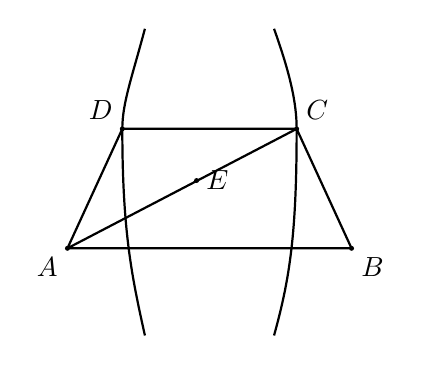
\begin{tikzpicture}[>=stealth, scale=0.82]
  \coordinate (A) at (0,0);
  \coordinate (B) at (4.4,0);
  \coordinate (D) at (0.85,1.85);
  \coordinate (C) at (3.55,1.85);
  \coordinate (E) at (2.0,1.05);

  \draw[thick] (A)--(B)--(C)--(D)--cycle;
  \draw[thick] (A)--(C);
  \draw[thick] (1.2,3.4) .. controls (1.0,2.65) and (0.85,2.25) .. (0.85,1.85);
  \draw[thick] (3.2,3.4) .. controls (3.45,2.7) and (3.55,2.25) .. (3.55,1.85);
  \draw[thick] (1.2,-1.35) .. controls (1.0,-0.45) and (0.85,0.25) .. (0.85,1.85);
  \draw[thick] (3.2,-1.35) .. controls (3.45,-0.45) and (3.55,0.25) .. (3.55,1.85);

  \fill (A) circle (1.1pt) node[below left] {$A$};
  \fill (B) circle (1.1pt) node[below right] {$B$};
  \fill (C) circle (1.1pt) node[above right] {$C$};
  \fill (D) circle (1.1pt) node[above left] {$D$};
  \fill (E) circle (1.1pt) node[right] {$E$};
\end{tikzpicture}
\end{center}
\nopagebreak[4]
\Needspace{4\baselineskip}
\textbf{解析}

\Needspace{5\baselineskip}
设双曲线的两个焦点为 $A,B$，令

\nopagebreak[4]
\[
AB=2c,\qquad
\text{\text{双曲线的实半轴}}=u,\qquad
\text{\text{虚半轴}}^2=c^2-u^2.
\]

\Needspace{5\baselineskip}
由 $AB=2CD$ 得 $CD=c$。取焦点坐标

\nopagebreak[4]
\[
A=(0,0),\qquad B=(2c,0),
\]

\Needspace{5\baselineskip}
双曲线中心为 $(c,0)$。由于 $C,D$ 在同一条与 $AB$ 平行的直线上且分居两支，可设

\nopagebreak[4]
\[
C=(c+uq,h),\qquad D=(c-uq,h),
\]

\Needspace{5\baselineskip}
其中

\nopagebreak[4]
\[
q=\sqrt{1+\frac{h^2}{c^2-u^2}}.
\]

\Needspace{5\baselineskip}
由 $CD=2uq=c$，得 $q=c/(2u)$，从而

\nopagebreak[4]
\[
C=\left(\frac{3c}{2},h\right).
\]

\Needspace{5\baselineskip}
设 $E$ 分有向线段 $AC$ 所成的比为

\nopagebreak[4]
\[
\frac{AE}{EC}=\lambda,
\qquad
s=\frac{\lambda}{1+\lambda},
\]

\Needspace{5\baselineskip}
则 $E=sC$。把 $E$ 代入双曲线方程

\nopagebreak[4]
\[
\frac{(x-c)^2}{u^2}-\frac{y^2}{c^2-u^2}=1
\]

\Needspace{5\baselineskip}
并利用 $C$ 在双曲线上，可化为

\nopagebreak[4]
\[
(s-1)\left[(2s-1)+\frac{u^2}{c^2}(s+1)\right]=0.
\]

\Needspace{5\baselineskip}
因 $E\ne C$，故

\nopagebreak[4]
\[
\frac{u^2}{c^2}
=\frac{1-2s}{s+1}
=\frac{1-\lambda}{1+3\lambda}.
\]

\Needspace{5\baselineskip}
双曲线离心率为 $e=c/u$，所以

\nopagebreak[4]
\[
e=\sqrt{\frac{1+3\lambda}{1-\lambda}}.
\]

\Needspace{5\baselineskip}
在 $\dfrac23\le\lambda\le\dfrac34$ 上，该式递增，故

\nopagebreak[4]
\[
e_{\min}=3,\qquad e_{\max}=\sqrt{13}.
\]

\Needspace{5\baselineskip}
因此

\nopagebreak[4]
\[
3\le e\le\sqrt{13}.
\]

\gkanswer{答案：$3\le e\le\sqrt{13}$}

\end{answer}